% Provenance (never printed): old premiere S material on the formation of fossil
% fuels (preserved organic matter, burial, oil window, migration, trap, coal).
% Burial history of the invented Merrow Basin from figdata/grade-11/oil_window.py
% (constant geotherm, no compaction). Rifts and passive margins after the USGS
% West-Central Coastal Province fact sheet (2023-3028). Folds are defined in
% g12.02 mountain-building (Sync 0): the anticline is told in prose here, never
% defined. Sedimentary basins compared, diagenesis: Year 1/2.
\chapter{La géologie du charbon, du pétrole et du gaz}\label{ch:g11:fossil-fuel-geology}

Une plaque d'argilite noire tirée d'une ancienne mine de \omterm{def:g11:fossil-fuel-geology:coal}{charbon} de
Pennsylvanie porte des feuilles de plantes semblables à des fougères,
aplaties et argentées sur la roche sombre. Elles ont poussé dans un marais
il y a plus de trois cents millions d'années, au Carbonifère~; enfouies
avant d'avoir pu pourrir, elles ont gardé leur forme, et le carbone des
plantes du marais est devenu du \omterm{def:g11:fossil-fuel-geology:coal}{charbon}. Le pétrole et le gaz, pompés
aujourd'hui depuis des plates-formes en mer, ont une origine du même
genre~: les restes d'êtres vivants qui ont échappé à la décomposition, puis
ont été enfouis et chauffés. Ce chapitre suit ce carbone enfoui, du marais
et du fond de la mer jusqu'à la veine de \omterm{def:g11:fossil-fuel-geology:coal}{charbon} et au gisement de pétrole.
% ledger: photo:g11-fossil-plants, ics:base.Carboniferous, ics:base.Permian, earle:coal-formation, earle:organic-preservation

\begin{omfigure}
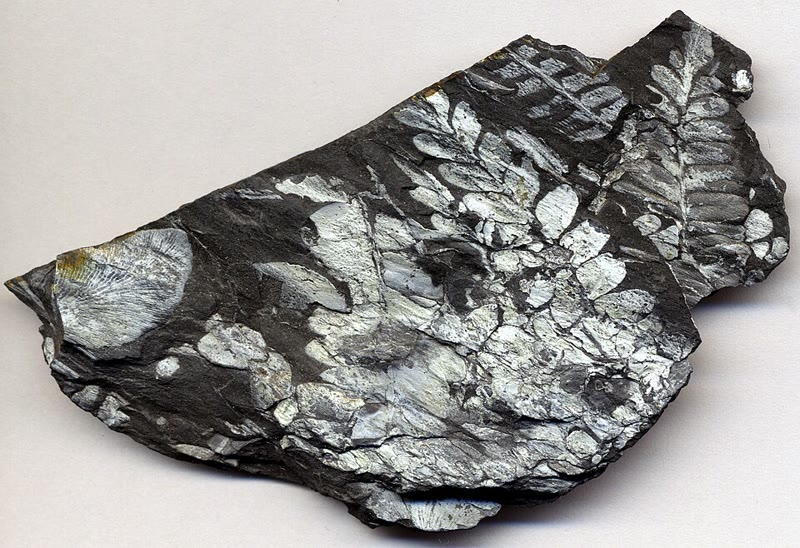
\includegraphics[height=4.4cm]{images/book2/g11-stjohn-fossil-plants.jpg}\hspace{0.03\linewidth}%
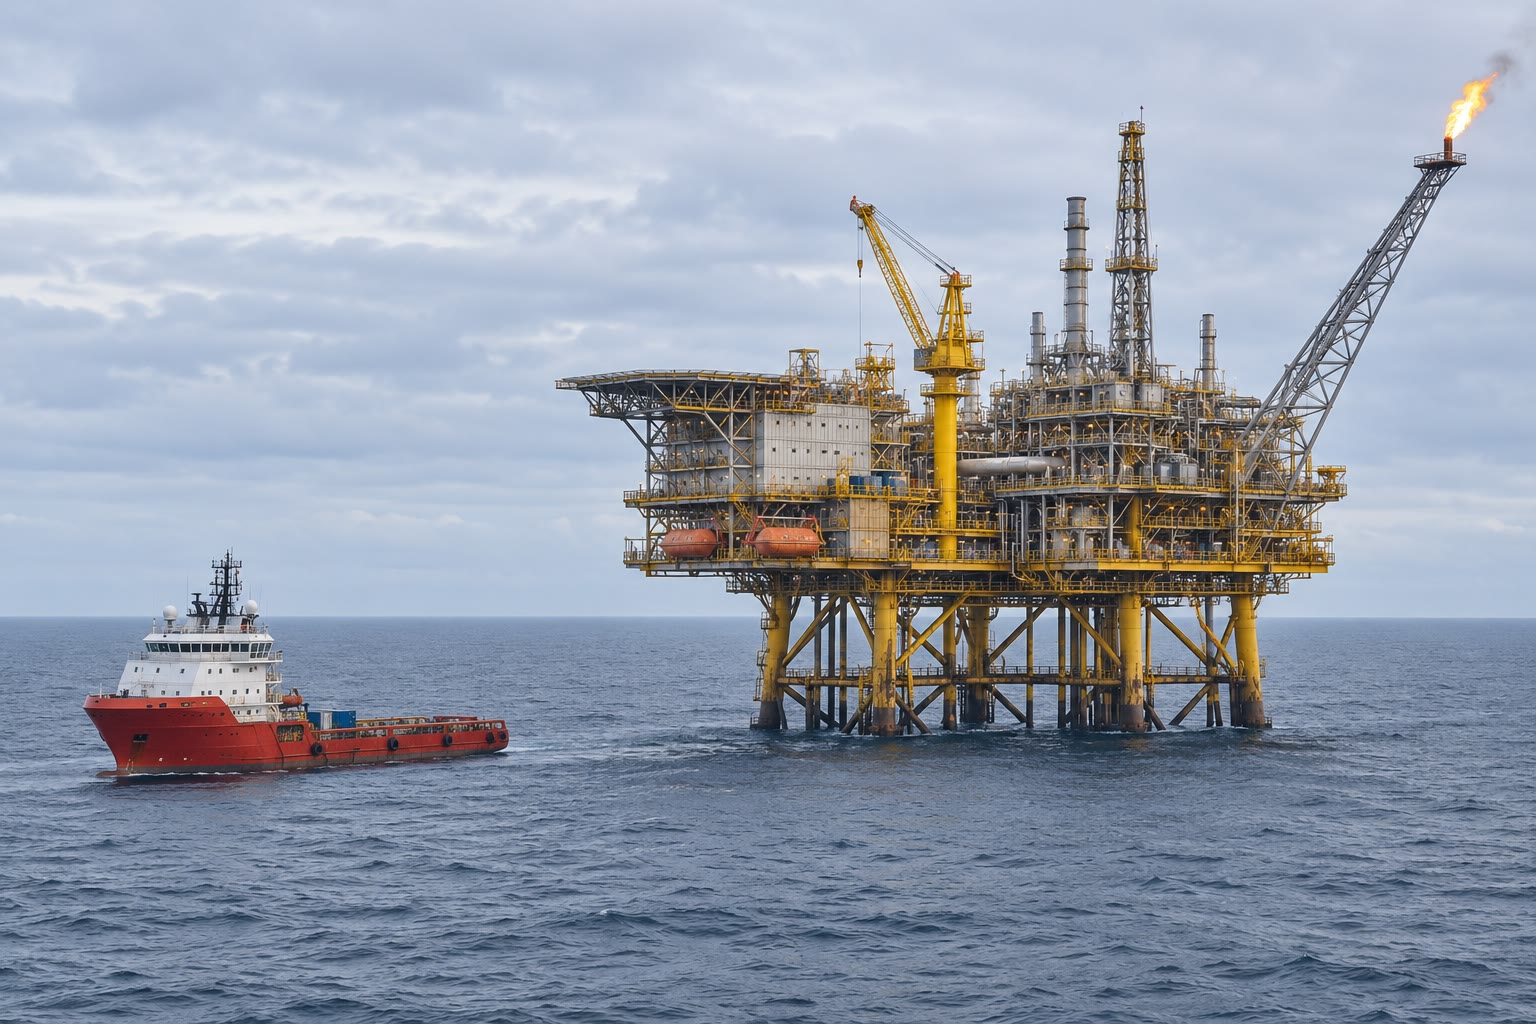
\includegraphics[height=4.4cm]{images/book2/ai/g11-offshore-platform.jpg}

{\small À gauche~: feuilles de plantes fossiles dans une argilite riche en
carbone provenant d'une ancienne mine de \omterm{def:g11:fossil-fuel-geology:coal}{charbon} de Pennsylvanie, du
Carbonifère~; la plaque mesure environ \qty{10}{cm} de large. Photographie
James St.~John (CC~BY~2.0). À droite~: une plate-forme de production de
pétrole et de gaz en mer (illustration générée par IA).}
\end{omfigure}
% ledger: photo:g11-fossil-plants

\begin{recall}
Le \omterm{def:g11:fossil-fuel-geology:coal}{charbon}, le pétrole et le gaz naturel sont des combustibles fossiles~:
le pétrole et le gaz sont des mélanges d'hydrocarbures, des composés de
carbone et d'hydrogène, et brûler un combustible fossile libère de
l'énergie et du dioxyde de carbone (les livres de chimie). Les plantes et
les algues fabriquent de la matière organique à partir de dioxyde de
carbone et d'eau par la photosynthèse (les livres de biologie). Le \omterm{def:g11:fossil-fuel-geology:coal}{charbon},
le pétrole et le gaz viennent de matière organique enfouie dans des
sédiments, et ils sont stockés dans des roches sédimentaires (livre~1,
année~9). Une roche est poreuse quand elle contient des vides, perméable
quand l'eau peut la traverser (livre~1, année~6). La température augmente
avec la profondeur le long du \omterm{def:g11:lithosphere-asthenosphere:geotherm}{géotherme}, de 25 à \qty{30}{\degreeCelsius}
par kilomètre dans les premiers kilomètres
(\cref{ch:g11:lithosphere-asthenosphere}).
\end{recall}
% ledger: usgs:gradient-29, earle:organic-preservation

\section{Conserver la matière organique}

La plus grande partie de la matière organique ne devient jamais un
combustible. Une feuille morte ou une algue morte est mangée par des
animaux et des bactéries, ou réagit avec l'oxygène de l'air~: en quelques
semaines ou quelques années, son carbone est retourné dans l'atmosphère
sous forme de dioxyde de carbone. La matière organique ne survit que là où
elle est coupée de l'oxygène --- au fond d'un marais aux eaux stagnantes,
ou sur un fond marin ou lacustre dont l'eau ne contient pas d'oxygène.
Enfouie là sous d'autres sédiments, elle peut se conserver pendant des
dizaines ou des centaines de millions d'années.
% ledger: earle:organic-preservation

Le \omterm{def:g11:fossil-fuel-geology:coal}{charbon} vient surtout de plantes terrestres accumulées dans des marais.
Le pétrole et le gaz viennent surtout des algues microscopiques et des
autres organismes du plancton marin~: là où les eaux de surface sont très
productives, le plancton mort tombe sur le fond assez vite pour qu'une
partie échappe à la décomposition, et il est enfoui dans la boue.
% ledger: earle:coal-formation, earle:oil-window

\begin{definition}[Roche mère~; kérogène]\label{def:g11:fossil-fuel-geology:source-rock}
Le \emph{kérogène}\index{kerogene@kérogène} est la matière organique
dispersée dans une roche sédimentaire, en petites particules qui ne se
dissolvent pas dans les solvants organiques. Une \emph{roche
mère}\index{roche mere (petroliere)@roche mère (pétrolière)} est une roche
sédimentaire riche en kérogène, dans laquelle le pétrole et le gaz se
forment quand elle est enfouie et chauffée.
\end{definition}
% ledger: peters08:kerogen, earle:migration-traps

La plupart des \omterm{def:g11:fossil-fuel-geology:source-rock}{roches mères} sont des argilites et des pélites, déposées
sous forme de boues riches en matière organique. Près de la surface, leur
\omterm{def:g11:fossil-fuel-geology:source-rock}{kérogène} reste solide~: des bactéries vivant sans oxygène transforment une
partie de la matière organique en méthane, mais la plus grande partie de ce
méthane s'échappe vers la surface. Fabriquer du pétrole demande de la
chaleur, et la chaleur demande de la profondeur.
% ledger: earle:oil-window, peters08:kerogen

\section{Enfouissement et maturation}

\begin{definition}[Bassin sédimentaire]\label{def:g11:fossil-fuel-geology:basin}
Un \emph{bassin sédimentaire}\index{bassin sedimentaire@bassin sédimentaire}
est une région de la croûte qui s'enfonce pendant des millions d'années, si
bien que des sédiments s'y accumulent, souvent sur plusieurs kilomètres
d'épaisseur.
\end{definition}
% ledger: usgs23:rift-salt

Dans un bassin qui s'enfonce, chaque couche est enfouie de plus en plus
profondément sous les couches qui s'empilent sur elle. En descendant, elle
suit le \omterm{def:g11:lithosphere-asthenosphere:geotherm}{géotherme}~: elle est chauffée. Son \omterm{def:g11:fossil-fuel-geology:source-rock}{kérogène} cuit lentement, ses
grosses molécules se cassant en molécules plus petites, celles du pétrole
et du gaz.
% ledger: earle:oil-window

\begin{definition}[Maturation~; fenêtre à huile~; fenêtre à gaz]\label{def:g11:fossil-fuel-geology:oil-window}
La \emph{maturation}\index{maturation} d'une \omterm{def:g11:fossil-fuel-geology:source-rock}{roche mère} est la
transformation de son \omterm{def:g11:fossil-fuel-geology:source-rock}{kérogène} en pétrole et en gaz à mesure qu'elle est
enfouie et chauffée. La \emph{fenêtre à huile}\index{fenetre a huile@fenêtre à huile}
est l'intervalle de température, d'environ 60 à
\qty{120}{\degreeCelsius}, dans lequel le \omterm{def:g11:fossil-fuel-geology:source-rock}{kérogène} forme surtout du
pétrole. Au-delà d'environ \qty{120}{\degreeCelsius}, dans la
\emph{fenêtre à gaz}\index{fenetre a gaz@fenêtre à gaz}, il forme surtout
du méthane.
\end{definition}
% ledger: earle:oil-window, magoon00:tps

Comme la température augmente avec la profondeur, la \omterm{def:g11:fossil-fuel-geology:oil-window}{fenêtre à huile} est
aussi un intervalle de profondeurs. Là où le \omterm{def:g11:lithosphere-asthenosphere:geotherm}{géotherme} est une droite, on
la trouve facilement.

\begin{proposition}[Profondeur de la fenêtre à huile]\label{prop:g11:fossil-fuel-geology:window-depth}
Supposons que la température vaille $T_0$ en surface et augmente avec la
profondeur $z$ selon un \omterm{def:g11:lithosphere-asthenosphere:geotherm}{gradient géothermique} constant $G$~:
$T = T_0 + G z$. La \omterm{def:g11:fossil-fuel-geology:oil-window}{fenêtre à huile} se trouve alors entre les profondeurs
\[
  z_{\text{sommet}} = \frac{60 - T_0}{G}
  \qquad\text{et}\qquad
  z_{\text{base}} = \frac{120 - T_0}{G},
\]
les températures étant en \unit{\degreeCelsius}. Son épaisseur vaut
$60/G$~: plus le \omterm{def:g11:lithosphere-asthenosphere:geotherm}{géotherme} est raide, moins la fenêtre est profonde et
épaisse.
\end{proposition}
% ledger: earle:oil-window

\begin{proof}
Le sommet de la fenêtre est la profondeur où $T_0 + G z = 60$,
c'est-à-dire $z = (60 - T_0)/G$~; la base est là où $T_0 + G z = 120$.
La différence vaut $(120 - 60)/G = 60/G$.
\end{proof}

Avec une surface à \qty{20}{\degreeCelsius} et un gradient de
\qty{30}{\degreeCelsius} par kilomètre, la \omterm{def:g11:fossil-fuel-geology:oil-window}{fenêtre à huile} se trouve entre
$40/30 \approx \qty{1.3}{km}$ et $100/30 \approx \qty{3.3}{km}$. Dans les
forages des États-Unis, le gradient vaut en moyenne
\qty{29}{\degreeCelsius} par kilomètre, \num{25} dans l'Est et \num{34}
dans l'Ouest~; une \omterm{def:g11:fossil-fuel-geology:source-rock}{roche mère} doit en général être enfouie à plus de
\qty{2}{km} environ avant de produire du pétrole. Faute de mesure sur le
\omterm{def:g11:fossil-fuel-geology:source-rock}{kérogène}, les géologues pétroliers ont considéré comme mature une \omterm{def:g11:fossil-fuel-geology:source-rock}{roche
mère} enfouie sous plus de \qty{3}{km} environ de roches plus jeunes.
% values (oil_window.py): z_top_km 1.3333, z_base_km 3.3333
% ledger: usgs:gradient-29, earle:oil-window, magoon00:tps

\begin{omfigure}
\begin{tikzpicture}
\begin{axis}[omrecord, omage, omdepth, name=burial, width=0.54\linewidth, height=5.6cm,
  xmin=0, xmax=170, ymin=0, ymax=4.5, xlabel={âge (millions d'années)},
  ylabel={profondeur (\unit{km})}, unbounded coords=jump, clip=false,
  xtick={0,20,...,160}, ytick={0,1,...,4}]
\fill[omProp!18] (axis cs:170,1.3333) rectangle (axis cs:0,3.3333);
\fill[omThm!12] (axis cs:170,3.3333) rectangle (axis cs:0,4.5);
\node[font=\scriptsize, anchor=west, text=omProp!80!black] at (axis cs:168,1.75) {fenêtre à huile};
\node[font=\scriptsize, anchor=west, text=omThm] at (axis cs:168,3.9) {fenêtre à gaz};
\node[font=\scriptsize, anchor=south west, text=black!60, inner sep=1pt] at (axis cs:168,1.3333) {\qty{60}{\degreeCelsius}};
\node[font=\scriptsize, anchor=south west, text=black!60, inner sep=1pt] at (axis cs:168,3.3333) {\qty{120}{\degreeCelsius}};
% computed in figdata/grade-11/oil_window.py (invented basin)
\addplot[black!45, line width=0.6pt] table[x=age, y=z150] {figdata/out/grade-11-oil_window-history.dat};
\addplot[black!45, line width=0.6pt] table[x=age, y=z120] {figdata/out/grade-11-oil_window-history.dat};
\addplot[black!45, line width=0.6pt] table[x=age, y=z95] {figdata/out/grade-11-oil_window-history.dat};
\addplot[black!45, line width=0.6pt] table[x=age, y=z66] {figdata/out/grade-11-oil_window-history.dat};
\addplot[black, line width=1.4pt] table[x=age, y=z165] {figdata/out/grade-11-oil_window-history.dat};
\draw[omDef, dashed, line width=0.8pt] (axis cs:80,0) -- (axis cs:80,4.5);
\node[font=\scriptsize, anchor=west, text=omDef, inner sep=1pt] at (axis cs:78,4.2) {formation de l'anticlinal};
\fill[omThm] (axis cs:116.97,1.3333) circle (2pt);
\fill[omThm] (axis cs:51.24,3.3333) circle (2pt);
\node[font=\scriptsize, anchor=north east, inner sep=1pt] at (axis cs:100,2.3) {roche mère};
\end{axis}
\begin{axis}[omrecord, omdepth, at={(burial.east)}, anchor=west, xshift=1.7cm, width=0.34\linewidth, height=5.6cm,
  xmin=15, xmax=50, ymin=0, ymax=7, xlabel={gradient (\unit{\degreeCelsius/km})},
  ylabel={profondeur (\unit{km})}]
% computed in figdata/grade-11/oil_window.py (proposition, surface at 20 degC)
\addplot[name path=top, omProp, line width=1pt] table[x=G, y=z_top] {figdata/out/grade-11-oil_window-windows.dat};
\addplot[name path=base, omThm, line width=1pt] table[x=G, y=z_base] {figdata/out/grade-11-oil_window-windows.dat};
\addplot[omProp!18] fill between[of=top and base];
\node[font=\scriptsize] at (axis cs:40,1.75) {fenêtre à huile};
\node[font=\scriptsize, anchor=south, text=omProp!80!black] at (axis cs:42,0.95) {sommet};
\node[font=\scriptsize, anchor=north west, text=omThm] at (axis cs:24,4.6) {base};
\end{axis}
\end{tikzpicture}

{\small À gauche~: histoire de l'enfouissement du bassin de Merrow, un
bassin inventé (modèle calculé, sans tenir compte de la compaction).
Chaque courbe suit une couche au cours du temps, depuis le jour où elle
s'est déposée en surface~; la courbe épaisse est la \omterm{def:g11:fossil-fuel-geology:source-rock}{roche mère}, déposée il
y a 165 millions d'années. Avec une surface à \qty{20}{\degreeCelsius} et
un gradient de \qty{30}{\degreeCelsius} par kilomètre, la \omterm{def:g11:fossil-fuel-geology:oil-window}{fenêtre à huile}
est la bande comprise entre \num{1.3} et \qty{3.3}{km}. Les points marquent
le moment où la \omterm{def:g11:fossil-fuel-geology:source-rock}{roche mère} y est entrée et celui où elle l'a quittée, pour
la \omterm{def:g11:fossil-fuel-geology:oil-window}{fenêtre à gaz}. À droite~: profondeur du sommet et de la base de la
\omterm{def:g11:fossil-fuel-geology:oil-window}{fenêtre à huile} en fonction du \omterm{def:g11:lithosphere-asthenosphere:geotherm}{gradient géothermique} (surface à
\qty{20}{\degreeCelsius}).}
\end{omfigure}
% values (oil_window.py): enter_oil_Ma 116.97, leave_oil_Ma 51.24, T_max 140 (20 Ma), T_today 125

Un tel diagramme est un \emph{diagramme d'enfouissement}~: l'âge y va de
gauche à droite jusqu'à aujourd'hui, la profondeur vers le bas. Il
transforme une colonne de roches, datée couche par couche, en une histoire.

\begin{method}[Lire un diagramme d'enfouissement]\label{met:g11:fossil-fuel-geology:burial}
\begin{enumerate}
  \item Repérer la courbe de la \omterm{def:g11:fossil-fuel-geology:source-rock}{roche mère}~: elle part de la surface le
        jour où la roche s'est déposée.
  \item Tracer le sommet et la base de la \omterm{def:g11:fossil-fuel-geology:oil-window}{fenêtre à huile}, en profondeur,
        à partir du \omterm{def:g11:lithosphere-asthenosphere:geotherm}{géotherme}
        (\cref{prop:g11:fossil-fuel-geology:window-depth}).
  \item Lire l'âge auquel la courbe de la \omterm{def:g11:fossil-fuel-geology:source-rock}{roche mère} croise le sommet de la
        fenêtre~: la \omterm{def:g11:fossil-fuel-geology:source-rock}{roche mère} commence à produire du pétrole. Lire l'âge
        auquel elle croise la base~: à partir de là, elle produit du gaz.
  \item Comparer ces âges à celui du \omterm{def:g11:fossil-fuel-geology:trap}{piège}~: seuls le pétrole et le gaz
        formés après l'apparition du \omterm{def:g11:fossil-fuel-geology:trap}{piège} peuvent y être retenus.
\end{enumerate}
\end{method}
% ledger: magoon00:tps

Dans le bassin de Merrow, la \omterm{def:g11:fossil-fuel-geology:source-rock}{roche mère} entre dans la \omterm{def:g11:fossil-fuel-geology:oil-window}{fenêtre à huile} il y
a environ 117 millions d'années et en sort il y a environ 51 millions
d'années~; son enfouissement maximal, \qty{4.0}{km} à
\qty{140}{\degreeCelsius}, date d'il y a 20 millions d'années, avant que le
soulèvement et l'érosion la fassent remonter. Aujourd'hui, elle est
toujours dans la \omterm{def:g11:fossil-fuel-geology:oil-window}{fenêtre à gaz}. Le problème du week-end calcule ces âges.
% values (oil_window.py): enter_oil_Ma 116.97, leave_oil_Ma 51.24, z_max_km 4, T_max 140, T_today 125

\section{De la roche mère au piège}

Le pétrole et le gaz sont plus légers que l'eau, et les pores des roches
enfouies sont pleins d'eau. Une fois formés, ils sont chassés de la \omterm{def:g11:fossil-fuel-geology:source-rock}{roche
mère} et remontent lentement à travers toute roche qui les laisse passer.
% ledger: earle:migration-traps

\begin{definition}[Migration]\label{def:g11:fossil-fuel-geology:migration}
La \emph{migration}\index{migration (du petrole et du gaz)@migration (du pétrole et du gaz)}
est le lent déplacement du pétrole et du gaz hors de la \omterm{def:g11:fossil-fuel-geology:source-rock}{roche mère} où ils
se sont formés, vers le haut à travers des roches perméables, sous l'effet
de leur densité plus faible que celle de l'eau qui les entoure.
\end{definition}
% ledger: earle:migration-traps

\begin{definition}[Roche réservoir~; roche couverture]\label{def:g11:fossil-fuel-geology:reservoir}
Une \emph{roche réservoir}\index{roche reservoir@roche réservoir} est une
roche poreuse et perméable dans laquelle le pétrole et le gaz
s'accumulent~: ses pores les stockent, et leurs connexions les laissent
s'écouler vers un puits. Une \emph{roche couverture}\index{roche couverture}
est une roche imperméable située au-dessus du réservoir, que le pétrole et
le gaz ne peuvent pas traverser.
\end{definition}
% ledger: earle:migration-traps, magoon00:tps

Les grès et certains calcaires font de bons réservoirs~; les pélites, les
argilites et le sel font de bonnes \omterm{def:g11:fossil-fuel-geology:reservoir}{couvertures}. Là où rien ne les arrête, le
pétrole et le gaz atteignent la surface, où ils suintent et sont oxydés~:
leur carbone retourne dans l'atmosphère. Ils ne s'accumulent que là où une
\omterm{def:g11:fossil-fuel-geology:reservoir}{couverture} a une forme telle qu'ils ne peuvent pas la contourner.
% ledger: earle:migration-traps, magoon00:tps

\begin{definition}[Piège]\label{def:g11:fossil-fuel-geology:trap}
Un \emph{piège}\index{piege (petrole et gaz)@piège (pétrole et gaz)} est un
agencement de \omterm{def:g11:fossil-fuel-geology:reservoir}{roche réservoir} et de \omterm{def:g11:fossil-fuel-geology:reservoir}{roche couverture} qui retient le pétrole
et le gaz en place, en leur fermant la route vers le haut de tous les
côtés.
\end{definition}
% ledger: earle:migration-traps

\begin{omfigure}
\begin{tikzpicture}[font=\footnotesize, scale=0.95,
    declare function={hz(\x,\c)=\c+0.1*\x+0.7*exp(-((\x-10)^2)/2.5);}]
  \colorlet{omOil}{green!45!black}\colorlet{omGas}{red!65}
  \fill[omLithShale!70!white] (0,0) rectangle (14,-6.3);
  % overburden: limestone above a sandstone
  \fill[omLithCongl!70!white] (0,0) -- (14,0) -- plot[domain=14:0, samples=80] (\x,{-2.4+0.06*\x+0.3*exp(-((\x-10)^2)/2.5)}) -- cycle;
  \fill[omLithSand!60!white] plot[domain=0:14, samples=80] (\x,{-2.4+0.06*\x+0.3*exp(-((\x-10)^2)/2.5)}) -- plot[domain=14:0, samples=80] (\x,{hz(\x,-3.7)}) -- cycle;
  % seal (mudstone)
  \fill[omLithShale] plot[domain=0:14, samples=80] (\x,{hz(\x,-3.7)}) -- plot[domain=14:0, samples=80] (\x,{hz(\x,-4.4)}) -- cycle;
  % reservoir sandstone
  \fill[omLithSand] plot[domain=0:14, samples=80] (\x,{hz(\x,-4.4)}) -- plot[domain=14:0, samples=80] (\x,{hz(\x,-5.0)}) -- cycle;
  % oil and gas in the crest of the anticline, above the spill depth
  \begin{scope}
    \clip plot[domain=0:14, samples=80] (\x,{hz(\x,-4.4)}) -- plot[domain=14:0, samples=80] (\x,{hz(\x,-5.0)}) -- cycle;
    \fill[omOil] (8,-2.97) rectangle (13,-2.6);
    \fill[omGas] (8,-2.81) rectangle (13,-2.6);
  \end{scope}
  % source rock (black shale)
  \fill[black!70] plot[domain=0:14, samples=80] (\x,{hz(\x,-5.0)}) -- plot[domain=14:0, samples=80] (\x,{hz(\x,-5.6)}) -- cycle;
  \foreach \c in {-3.7,-4.4,-5.0,-5.6}
    \draw[black!55, line width=0.4pt] plot[domain=0:14, samples=80] (\x,{hz(\x,\c)});
  \draw[black!55, line width=0.4pt] plot[domain=0:14, samples=80] (\x,{-2.4+0.06*\x+0.3*exp(-((\x-10)^2)/2.5)});
  \draw[black!70] (0,0) -- (14,0);
  % 60 degC isotherm
  \draw[omThm, dashed, line width=0.8pt] (0,-4.3) -- (14,-4.3);
  \node[anchor=north east, text=omThm, fill=omLithShale!70!white, inner sep=1pt] at (13.95,-4.35) {\qty{60}{\degreeCelsius}};
  % migration
  \foreach \s in {0,1}
    \draw[->, omDef, line width=1.1pt] (2.7+1.2*\s,{-5.1+0.12*\s}) -- (3.2+1.2*\s,{-4.55+0.12*\s});
  \draw[->, omDef, line width=1.1pt] (4.6,-4.3) .. controls (6.5,-4.1) and (8.3,-3.7) .. (9.45,-3.0);
  % labels
  \node[anchor=west, text=white] at (0.15,-5.25) {roche mère};
  \node[anchor=west] at (5.2,-5.75) {mature au-delà de \qty{60}{\degreeCelsius}};
  \node[anchor=west] at (0.15,-4.75) {roche réservoir};
  \node[anchor=west] at (0.15,-3.97) {couverture};
  \node[anchor=west] at (0.15,-0.4) {roches de recouvrement};
  \node[anchor=north, text=omDef, fill=omLithShale, inner sep=1pt] at (6.2,-3.62) {migration};
  \draw[black!60] (10.0,-2.72) -- (11.4,-1.95);
  \node[anchor=south west, fill=omLithSand!60!white, inner sep=1pt] at (11.4,-1.95) {gaz};
  \draw[black!60] (10.6,-2.88) -- (12.3,-2.55);
  \node[anchor=west, fill=omLithShale, inner sep=1pt] at (12.3,-2.55) {pétrole};
  \draw[black!60] (12.0,-3.45) -- (12.8,-3.15);
  \node[anchor=south, fill=omLithShale, inner sep=1pt] at (12.85,-3.15) {eau};
  \node[anchor=north] at (10,-1.0) {piège~: la voûte d'un anticlinal};
\end{tikzpicture}

{\small Un \omterm{def:g11:fossil-fuel-geology:petroleum-system}{système pétrolier} (dessin sans échelle). La \omterm{def:g11:fossil-fuel-geology:source-rock}{roche mère},
profonde, à gauche, se trouve sous l'isotherme \qty{60}{\degreeCelsius} et
produit du pétrole~; le pétrole et le gaz en sortent vers le grès situé
au-dessus et remontent lentement le long de celui-ci, sous la \omterm{def:g11:fossil-fuel-geology:reservoir}{couverture}
d'argilite, jusqu'à la voûte d'un anticlinal. Là, ils se rangent par
densité~: le gaz en haut, le pétrole au-dessous, l'eau en bas. Les \omterm{def:g11:fossil-fuel-geology:petroleum-system}{roches de
recouvrement}, au-dessus, enfouissent la \omterm{def:g11:fossil-fuel-geology:source-rock}{roche mère} assez profondément pour
la rendre mature.}
\end{omfigure}
% ledger: earle:migration-traps, magoon00:tps, earle:oil-window

Dans un \omterm{def:g11:fossil-fuel-geology:trap}{piège}, les fluides se rangent par densité~: le gaz en haut, le
pétrole au-dessous, l'eau tout en bas. Le \omterm{def:g11:fossil-fuel-geology:trap}{piège} le plus simple est un
anticlinal, une voûte formée par les couches (les plis sont l'objet du
\cref{ch:g12:mountain-building}). Les failles, les dômes de sel et les
variations des roches elles-mêmes forment aussi des \omterm{def:g11:fossil-fuel-geology:trap}{pièges}.
% ledger: earle:migration-traps

\begin{omfigure}
\begin{tikzpicture}[font=\footnotesize, scale=0.78]
  \colorlet{omOil}{green!45!black}\colorlet{omGas}{red!65}
  % (a) anticline
  \begin{scope}
    \fill[omLithShale] (0,0) rectangle (4,3);
    \fill[omLithSand] plot[domain=0:4, samples=50] (\x,{1.0+1.0*exp(-((\x-2)^2)/1.2)}) -- plot[domain=4:0, samples=50] (\x,{1.5+1.0*exp(-((\x-2)^2)/1.2)}) -- cycle;
    \begin{scope}
      \clip plot[domain=0:4, samples=50] (\x,{1.0+1.0*exp(-((\x-2)^2)/1.2)}) -- plot[domain=4:0, samples=50] (\x,{1.5+1.0*exp(-((\x-2)^2)/1.2)}) -- cycle;
      \fill[omOil] (0,1.75) rectangle (4,3); \fill[omGas] (0,2.25) rectangle (4,3);
    \end{scope}
    \draw[black!50] (0,0) rectangle (4,3);
    \node[anchor=north, text height=1.6ex, text depth=0.3ex] at (2,-0.05) {(a) anticlinal};
  \end{scope}
  % (b) fault
  \begin{scope}[xshift=4.6cm]
    \fill[omLithShale] (0,0) rectangle (4,3);
    \begin{scope}
      \clip (0,0) -- (2.9,0) -- (2.3,3) -- (0,3) -- cycle;
      \fill[omLithSand] (0,0.6) -- (4,1.8) -- (4,2.3) -- (0,1.1) -- cycle;
      \clip (0,0.6) -- (4,1.8) -- (4,2.3) -- (0,1.1) -- cycle;
      \fill[omOil] (0,1.45) rectangle (4,3); \fill[omGas] (0,1.75) rectangle (4,3);
    \end{scope}
    \begin{scope}
      \clip (2.9,0) -- (4,0) -- (4,3) -- (2.3,3) -- cycle;
      \fill[omLithSand] (0,-0.6) -- (4,0.6) -- (4,1.1) -- (0,-0.1) -- cycle;
    \end{scope}
    \draw[black, line width=1pt] (2.9,0) -- (2.3,3);
    \draw[black!50] (0,0) rectangle (4,3);
    \node[anchor=north, text height=1.6ex, text depth=0.3ex] at (2,-0.05) {(b) faille};
  \end{scope}
  % (c) salt dome
  \begin{scope}[xshift=9.2cm]
    \fill[omLithShale] (0,0) rectangle (4,3);
    \fill[omLithSand] (0,0.9) -- (1.0,1.2) -- (1.4,1.9) -- (1.4,2.4) -- (1.0,1.7) -- (0,1.4) -- cycle;
    \fill[omLithSand] (4,0.9) -- (3.0,1.2) -- (2.6,1.9) -- (2.6,2.4) -- (3.0,1.7) -- (4,1.4) -- cycle;
    \begin{scope}
      \clip (0,0.9) -- (1.0,1.2) -- (1.4,1.9) -- (1.4,2.4) -- (1.0,1.7) -- (0,1.4) -- cycle;
      \fill[omOil] (0,1.65) rectangle (1.4,3); \fill[omGas] (0,2.05) rectangle (1.4,3);
    \end{scope}
    \begin{scope}
      \clip (4,0.9) -- (3.0,1.2) -- (2.6,1.9) -- (2.6,2.4) -- (3.0,1.7) -- (4,1.4) -- cycle;
      \fill[omOil] (2.6,1.65) rectangle (4,3); \fill[omGas] (2.6,2.05) rectangle (4,3);
    \end{scope}
    \fill[omLithEvap, draw=black!60] (1.4,0) -- (1.4,2.4) .. controls (1.4,2.85) and (2.6,2.85) .. (2.6,2.4) -- (2.6,0) -- cycle;
    \node at (2,1.0) {sel};
    \draw[black!50] (0,0) rectangle (4,3);
    \node[anchor=north, text height=1.6ex, text depth=0.3ex] at (2,-0.05) {(c) dôme de sel};
  \end{scope}
  % (d) stratigraphic
  \begin{scope}[xshift=13.8cm]
    \fill[omLithShale] (0,0) rectangle (4,3);
    \fill[omLithSand] (0,0.6) -- (3.5,1.95) -- (0,1.3) -- cycle;
    \begin{scope}
      \clip (0,0.6) -- (3.5,1.95) -- (0,1.3) -- cycle;
      \fill[omOil] (0,1.45) rectangle (4,3); \fill[omGas] (0,1.7) rectangle (4,3);
    \end{scope}
    \draw[black!50] (0,0) rectangle (4,3);
    \node[anchor=north, text height=1.6ex, text depth=0.3ex] at (2,-0.05) {(d) biseau};
  \end{scope}
\end{tikzpicture}

{\small Quatre types de \omterm{def:g11:fossil-fuel-geology:trap}{pièges} (dessins sans échelle)~: le grès réservoir en
jaune, l'argilite \omterm{def:g11:fossil-fuel-geology:reservoir}{couverture} en gris-vert, le pétrole en vert, le gaz en
rouge. (a) La voûte d'un anticlinal. (b) Un réservoir incliné coupé par une
faille, contre une argilite de l'autre côté. (c) Des couches relevées
contre un dôme de sel qui monte. (d) Un grès qui s'amincit vers le haut de
la pente au sein d'une argilite~: un \omterm{def:g11:fossil-fuel-geology:trap}{piège} dû à une variation des roches
elles-mêmes.}
\end{omfigure}
% ledger: earle:migration-traps

\begin{example}[Un piège dans un anticlinal]\label{ex:g11:fossil-fuel-geology:anticline}
Une campagne sismique cartographie le toit d'un grès scellé par une
argilite. Il forme une voûte dont le sommet se trouve à \qty{1800}{m} sous
la surface. Autour du sommet, la courbe de niveau la plus profonde qui se
referme encore tout autour se trouve à \qty{2050}{m}~; au-dessous, le grès
s'ouvre sur le côté. Un puits foré au sommet trouve du gaz jusqu'à
\qty{1880}{m}. Quelle hauteur de colonne de pétrole et de gaz le \omterm{def:g11:fossil-fuel-geology:trap}{piège}
peut-il retenir, et quelle est l'épaisseur du pétrole~?

\emph{Solution.} Le pétrole et le gaz remplissent la voûte depuis le sommet
vers le bas~; ce qui descend sous la dernière courbe fermée s'échappe sur
le côté, au \emph{point de fuite}, et poursuit sa \omterm{def:g11:fossil-fuel-geology:migration}{migration}. La colonne
mesure au plus $2050 - 1800 = \qty{250}{m}$ de haut. Si le \omterm{def:g11:fossil-fuel-geology:trap}{piège} est
plein, le gaz occupe les $1880 - 1800 = \qty{80}{m}$ du haut et le pétrole
les $2050 - 1880 = \qty{170}{m}$ suivants, avec de l'eau au-dessous.
\end{example}
% invented numbers; ledger: earle:migration-traps

Chacune des pièces --- une \omterm{def:g11:fossil-fuel-geology:source-rock}{roche mère}, un réservoir, une \omterm{def:g11:fossil-fuel-geology:reservoir}{couverture}, les
roches situées au-dessus qui enfouissent la \omterm{def:g11:fossil-fuel-geology:source-rock}{roche mère}, un \omterm{def:g11:fossil-fuel-geology:trap}{piège} --- est
nécessaire, et elles doivent se mettre en place dans le bon ordre.

\begin{definition}[Système pétrolier]\label{def:g11:fossil-fuel-geology:petroleum-system}
Un \emph{système pétrolier}\index{systeme petrolier@système pétrolier} est
un ensemble de \omterm{def:g11:fossil-fuel-geology:source-rock}{roche mère} mature avec tout le pétrole et tout le gaz qui en
sont issus, ainsi que les éléments et les processus dont ils ont besoin~: la
\omterm{def:g11:fossil-fuel-geology:source-rock}{roche mère}, la \omterm{def:g11:fossil-fuel-geology:reservoir}{roche réservoir}, la \omterm{def:g11:fossil-fuel-geology:reservoir}{couverture} et les \emph{roches de
recouvrement}\index{roches de recouvrement} (les roches situées au-dessus,
qui enfouissent la \omterm{def:g11:fossil-fuel-geology:source-rock}{roche mère}), ainsi que la formation des \omterm{def:g11:fossil-fuel-geology:trap}{pièges}, la
génération, la \omterm{def:g11:fossil-fuel-geology:migration}{migration} et l'accumulation du pétrole et du gaz.
\end{definition}
% ledger: magoon00:tps

L'ordre est ce qui compte le plus. Un \omterm{def:g11:fossil-fuel-geology:trap}{piège} qui se forme après le passage du
pétrole ne retient rien~: le diagramme d'enfouissement date la génération
du pétrole, l'histoire des plis et des failles date le \omterm{def:g11:fossil-fuel-geology:trap}{piège}, et le \omterm{def:g11:fossil-fuel-geology:petroleum-system}{système
pétrolier} ne fonctionne que si le \omterm{def:g11:fossil-fuel-geology:trap}{piège} est venu en premier. Les géologues
pétroliers appellent aussi \emph{moment critique} l'époque qui montre le
mieux la génération, la \omterm{def:g11:fossil-fuel-geology:migration}{migration} et l'accumulation réunies.
% ledger: magoon00:tps

\section{Où le pétrole et le gaz s'accumulent}

Où un \omterm{def:g11:fossil-fuel-geology:petroleum-system}{système pétrolier} se met-il en place~? Il lui faut un bassin qui
s'enfonce longtemps, des eaux pauvres en oxygène pour conserver la matière
organique, et des \omterm{def:g11:fossil-fuel-geology:reservoir}{couvertures}. Les rifts et les marges continentales qu'ils
deviennent réunissent les trois.
% ledger: usgs23:rift-salt

Quand un continent commence à se fendre, comme l'Afrique aujourd'hui le
long du rift est-africain (livre~1, année~7), sa croûte s'étire et se
casse en blocs le long de \omterm{def:g11:ocean-ridges:normal-fault}{failles normales} (\cref{ch:g11:ocean-ridges}).
Certains blocs s'effondrent, d'autres basculent, et les fossés qui les
séparent se remplissent de sédiments, souvent sur plusieurs kilomètres
d'épaisseur, et de lacs, dont les boues riches en matière organique peuvent
devenir des \omterm{def:g11:fossil-fuel-geology:source-rock}{roches mères}. Quand l'étirement s'arrête, la croûte amincie
refroidit et continue de s'enfoncer lentement, si bien que le bassin
continue de se remplir. Si la mer envahit alors un bassin qui ne
communique qu'en partie avec l'océan et s'évapore, elle laisse d'épaisses
couches de sel. Une fois le rift ouvert en océan, ses bords deviennent des
marges passives~: des bordures de continent situées à l'intérieur d'une
plaque, loin de toute limite de plaques, qui continuent de s'enfoncer et de
recevoir des sédiments venus du continent.
% ledger: usgs23:rift-salt, usgs:pangaea-breakup

\begin{omfigure}
\begin{tikzpicture}[font=\footnotesize, x=1cm, y=0.8cm]
  \fill[omLithShale] (0,0.25) -- (1.5,0) -- (7,-0.4) -- (10,-2.2) -- (14,-2.6) -- (14,-8.0) -- (0,-8.0) -- cycle;
  % sea and land
  \fill[omSea] (1.5,0) -- (14,0) -- (14,-2.6) -- (10,-2.2) -- (7,-0.4) -- cycle;
  \draw[omRiver!60, line width=0.6pt] (1.5,0) -- (14,0);
  % marine sediments above the salt
  \fill[omLithShale] (0,0.25) -- (1.5,0) -- (7,-0.4) -- (10,-2.2) -- (14,-2.6) -- (14,-4.95) -- (11.2,-4.5) -- (11.2,-3.74) -- (0,-2.4) -- cycle;
  \fill[omLithSand] (0,-0.9) -- (6,-1.45) -- (10,-2.75) -- (14,-3.3) -- (14,-3.6) -- (10,-3.05) -- (6,-1.75) -- (0,-1.2) -- cycle;
  % salt layer and a salt dome
  \fill[omLithEvap, draw=black!50] (1.2,-2.25) -- (11.2,-3.74) -- (11.2,-4.14) -- (1.2,-2.65) -- cycle;
  \fill[omLithEvap, draw=black!50] (7.0,-3.0) .. controls (7.3,-2.6) and (7.25,-1.9) .. (7.2,-1.6)
     .. controls (7.4,-1.2) and (8.2,-1.2) .. (8.4,-1.6)
     .. controls (8.35,-2.1) and (8.3,-2.7) .. (8.7,-3.25) -- cycle;
  % continental crust with tilted blocks
  \fill[omLithGranite] (0,-2.75) -- (2.5,-3.0) -- (4.85,-4.6) -- (5.0,-3.4) -- (7.35,-5.0) -- (7.5,-3.75) -- (9.85,-5.3) -- (10.0,-4.1) -- (11.2,-5.0) -- (11.2,-6.0) -- (0,-7.6) -- cycle;
  % rift fill: lake shales (source rocks) in the half-grabens
  \fill[black!65] (2.5,-3.0) -- (4.85,-4.6) -- (5.0,-3.4) -- (4.0,-3.25) -- cycle;
  \fill[black!65] (5.0,-3.4) -- (7.35,-5.0) -- (7.5,-3.75) -- (6.5,-3.6) -- cycle;
  \fill[black!65] (7.5,-3.75) -- (9.85,-5.3) -- (10.0,-4.1) -- (9.0,-3.95) -- cycle;
  \fill[black!65] (2.5,-3.0) -- (4.0,-3.25) -- (5.0,-3.4) -- (6.5,-3.6) -- (7.5,-3.75) -- (9.0,-3.95) -- (10.0,-4.1) -- (11.2,-4.3) -- (11.2,-4.14) -- (1.2,-2.65) -- (1.2,-2.87) -- cycle;
  \draw[black!70, line width=0.8pt] (4.85,-4.6) -- (5.0,-3.4) (7.35,-5.0) -- (7.5,-3.75) (9.85,-5.3) -- (10.0,-4.1);
  % oceanic crust and mantle
  \fill[omLithBasalt] (11.2,-4.5) -- (14,-4.95) -- (14,-6.0) -- (11.2,-6.0) -- cycle;
  \fill[omLithPeridotite] (0,-7.6) -- (11.2,-6.0) -- (14,-6.0) -- (14,-8.0) -- (0,-8.0) -- cycle;
  % oil beside the salt dome
  \fill[green!45!black] (6.85,-1.5) -- (7.22,-1.65) -- (7.22,-1.95) -- (6.85,-1.75) -- cycle;
  \draw[black!60] (0,-8.0) rectangle (14,1.0);
  % labels
  \node[anchor=west] at (11.5,-1.2) {mer};
  \node[anchor=south west] at (0.1,0.3) {continent};
  \node[anchor=west, fill=omLithShale, inner sep=1pt] at (2.2,-0.45) {sédiments marins};
  \node[anchor=west, fill=omLithEvap, inner sep=1pt] at (9.0,-1.25) {dôme de sel};
  \draw[black!60] (8.4,-1.4) -- (9.0,-1.25);
  \node[anchor=east, fill=omLithShale, inner sep=1pt] at (6.6,-2.1) {pétrole};
  \draw[black!60] (6.6,-2.1) -- (6.95,-1.75);
  \node[anchor=west, fill=omLithShale, inner sep=1pt] at (11.4,-3.35) {sel (couverture)};
  \draw[black!60] (10.8,-3.7) -- (11.4,-3.35);
  \node[anchor=west, align=left] at (0.3,-4.7) {argilites lacustres\\(roches mères)};
  \draw[black!60] (2.75,-4.45) -- (4.4,-3.8);
  \node[anchor=north, align=center] at (4.0,-5.6) {croûte continentale étirée~:\\blocs basculés et failles normales};
  \node[anchor=north, align=center] at (12.6,-5.05) {croûte océanique};
  \node[anchor=north] at (6,-7.35) {manteau};
\end{tikzpicture}

{\small Une marge passive construite sur un ancien rift (dessin sans
échelle, profondeurs exagérées). Dans le rift, des blocs basculés de croûte
continentale limités par des \omterm{def:g11:ocean-ridges:normal-fault}{failles normales} contiennent des argilites
lacustres, les \omterm{def:g11:fossil-fuel-geology:source-rock}{roches mères}. Une couche de sel, déposée quand la jeune mer
s'est évaporée, les scelle~; au-dessus, des sédiments marins s'accumulent à
mesure que la marge s'enfonce. Le sel, plus léger que les sédiments qui
l'entourent, monte en dômes qui relèvent les couches en \omterm{def:g11:fossil-fuel-geology:trap}{pièges}.}
\end{omfigure}
% ledger: usgs23:rift-salt, earle:migration-traps

Les marges de l'Atlantique Sud se sont construites ainsi. L'Afrique et
l'Amérique du Sud ont commencé à se séparer à la fin du Trias ou au début
du Jurassique. Au large de l'Afrique centrale occidentale, les fossés du
rift se sont remplis de plusieurs kilomètres de sédiments, parmi lesquels
des argilites lacustres épaisses de jusqu'à \qty{600}{m}, contenant jusqu'à
\qty{20}{\percent} de carbone organique en masse. Au Crétacé inférieur, la
mer a commencé à envahir le bassin, encore et encore, et à s'évaporer, en
laissant plus d'un kilomètre de sel~; là où le sel est resté en place, il
scelle le pétrole et le gaz des roches situées au-dessous. Dans le golfe du
Mexique, du sel plus léger que les sédiments qui l'entourent est monté en
dômes, et les couches relevées contre eux forment des \omterm{def:g11:fossil-fuel-geology:trap}{pièges}.
% ledger: usgs23:rift-salt, earle:migration-traps

\section{Le charbon}

Le \omterm{def:g11:fossil-fuel-geology:coal}{charbon} se forme sur les continents, surtout dans des marais au bord des
rivières et des deltas, sous des climats humides, de tropicaux à tempérés,
là où les plantes poussent vite et où leurs restes tombent dans une eau
stagnante pauvre en oxygène. En quelques siècles ou quelques millénaires,
ils s'accumulent en tourbe. Quand une rivière change de cours, ou que la
mer monte, du sable et de la boue enfouissent la tourbe~; enfouie plus
profondément, elle est comprimée et chauffée.
% ledger: earle:coal-formation

\begin{definition}[Charbon~; houillification~; rang]\label{def:g11:fossil-fuel-geology:coal}
Le \emph{charbon}\index{charbon} est une roche sédimentaire formée surtout
de restes de plantes terrestres, riche en carbone. La
\emph{houillification}\index{houillification} est la transformation de la
tourbe en charbon, et d'un charbon en un charbon plus riche, par
enfouissement et chauffage. Le \emph{rang}\index{rang (d'un charbon)} d'un
charbon mesure l'avancement de la houillification~: du lignite à
l'anthracite, en passant par les charbons subbitumineux et bitumineux, la
teneur en carbone augmente.
\end{definition}
% ledger: earle:coal-formation, eia:coal-carbon

Le lignite se forme à des profondeurs allant de quelques centaines de
mètres à environ \qty{1.5}{km}, jusqu'à environ \qty{50}{\degreeCelsius}~;
le \omterm{def:g11:fossil-fuel-geology:coal}{charbon} bitumineux entre 1 et \qty{5}{km}, jusqu'à environ
\qty{150}{\degreeCelsius}~; l'anthracite au-delà de \qty{5}{km} et de
\qty{150}{\degreeCelsius}. À mesure que le \omterm{def:g11:fossil-fuel-geology:coal}{rang} augmente, le carbone forme
une part de plus en plus grande du \omterm{def:g11:fossil-fuel-geology:coal}{charbon}~: environ 25 à
\qty{35}{\percent} dans le lignite, jusqu'à 86 à \qty{97}{\percent} dans
l'anthracite. Le méthane formé en chemin reste dans les pores du \omterm{def:g11:fossil-fuel-geology:coal}{charbon},
ce qui explique qu'une mine de \omterm{def:g11:fossil-fuel-geology:coal}{charbon} puisse contenir un gaz explosif.
Former une veine de \omterm{def:g11:fossil-fuel-geology:coal}{charbon} demande des millions d'années.
% ledger: earle:coal-formation, eia:coal-carbon

\begin{omfigure}
\begin{tikzpicture}
\begin{axis}[omrecord, xbar, name=rank, width=0.5\linewidth, height=4.6cm, xmin=0, xmax=100,
  ymin=0.4, ymax=4.6, ytick={1,2,3,4},
  yticklabels={lignite, subbitumineux, bitumineux, anthracite},
  xlabel={teneur en carbone (\unit{\percent})}, ymajorgrids=false]
% ledger: eia:coal-carbon
\fill[omProp!60!black!35] (axis cs:25,0.7) rectangle (axis cs:35,1.3);
\fill[omProp!70!black!55] (axis cs:35,1.7) rectangle (axis cs:45,2.3);
\fill[black!60] (axis cs:45,2.7) rectangle (axis cs:86,3.3);
\fill[black!85] (axis cs:86,3.7) rectangle (axis cs:97,4.3);
\node[font=\scriptsize, anchor=west] at (axis cs:36,1) {25--35};
\node[font=\scriptsize, anchor=west] at (axis cs:46,2) {35--45};
\node[font=\scriptsize, anchor=east, text=white] at (axis cs:85,3) {45--86};
\node[font=\scriptsize, anchor=east] at (axis cs:85,4) {86--97};
\end{axis}
\node[anchor=west] at ([xshift=0.6cm]rank.east) {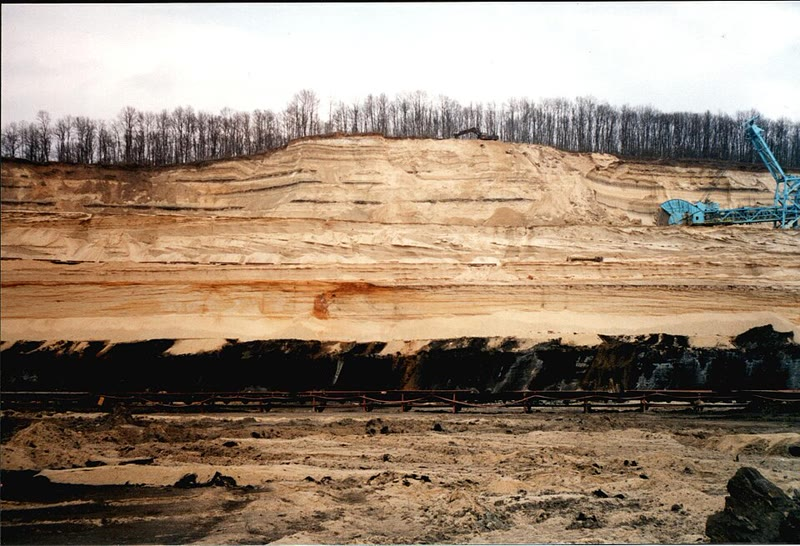
\includegraphics[height=4.0cm]{images/book2/g11-usgs-lignite-bed.jpg}};
\end{tikzpicture}

\medskip
\makebox[0.32\linewidth]{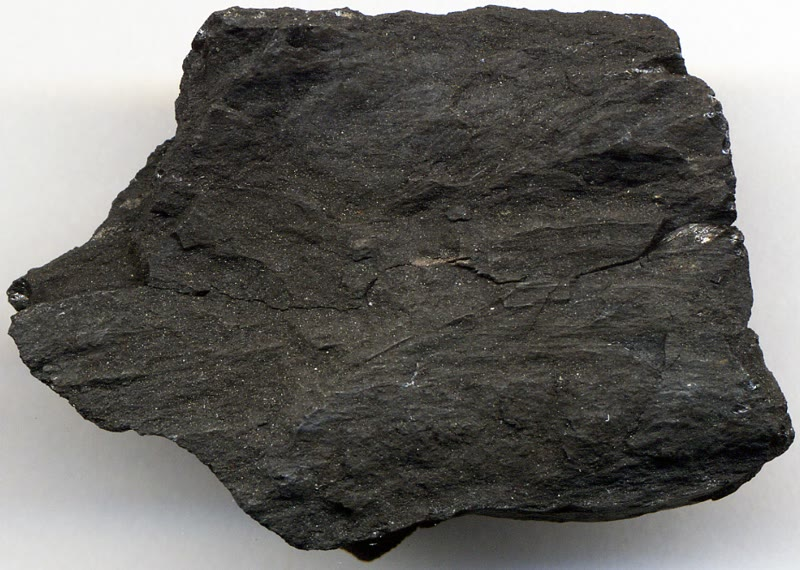
\includegraphics[height=3.2cm]{images/book2/g11-stjohn-lignite.jpg}}\hfill
\makebox[0.32\linewidth]{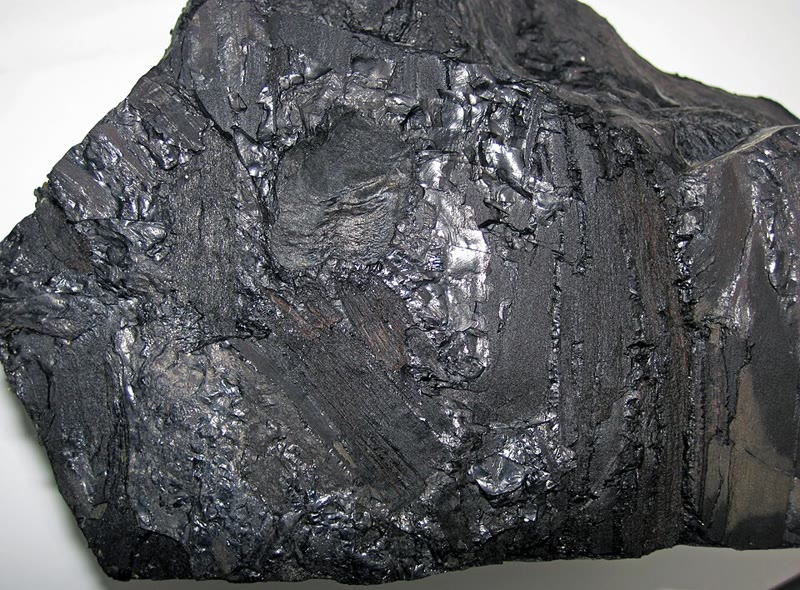
\includegraphics[height=3.2cm]{images/book2/g11-stjohn-bituminous.jpg}}\hfill
\makebox[0.32\linewidth]{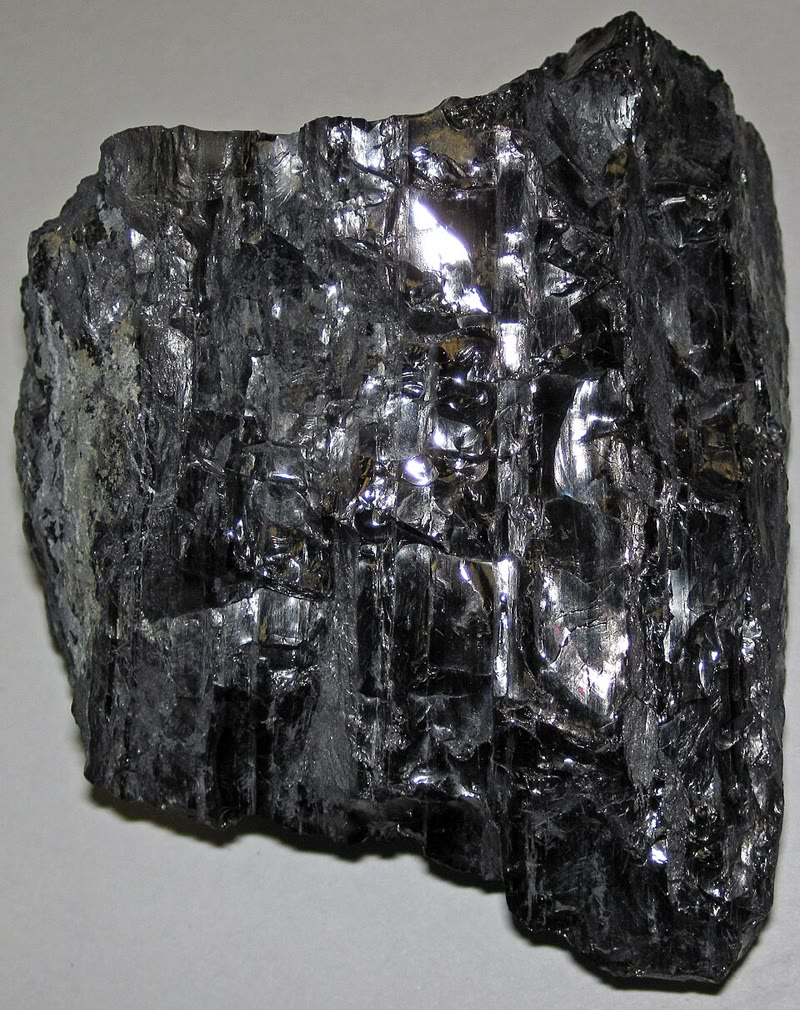
\includegraphics[height=3.2cm]{images/book2/g11-stjohn-anthracite.jpg}}

{\small En haut à gauche~: teneur en carbone des différents \omterm{def:g11:fossil-fuel-geology:coal}{rangs} de
\omterm{def:g11:fossil-fuel-geology:coal}{charbon}. Données~: U.S. Energy Information Administration. En haut à
droite~: une couche de lignite, la bande noire sous des sables pâles, mise
à nu dans une mine de Roumanie~; photographie U.S. Geological Survey
(domaine public). En bas, de gauche à droite~: un lignite, d'environ
\qty{4.5}{cm} de large, brun-noir et terne~; un \omterm{def:g11:fossil-fuel-geology:coal}{charbon} bitumineux, avec
des fragments de plantes aplatis~; un anthracite, noir et vitreux.
Photographies James St.~John (CC~BY~2.0).}
\end{omfigure}
% ledger: eia:coal-carbon, photo:g11-lignite-bed, photo:g11-coal-ranks

La tourbe perd l'essentiel de son volume en chemin. Dans une couche de
\omterm{def:g11:fossil-fuel-geology:coal}{charbon} du centre de l'Utah, la comparaison de la tourbe entaillée par un
ancien chenal de rivière avec le \omterm{def:g11:fossil-fuel-geology:coal}{charbon} qui manque à côté donne un rapport
des épaisseurs d'environ $11{:}1$~: chaque mètre de ce \omterm{def:g11:fossil-fuel-geology:coal}{charbon} bitumineux a
été autrefois quelque onze mètres de tourbe.
% ledger: ryer80:peat-coal

\section{Exercices}

\begin{exercise}[$\star$]\label{exo:g11:fossil-fuel-geology:1}
Remettre dans l'ordre les étapes qui mènent du plancton au pétrole dans un
\omterm{def:g11:fossil-fuel-geology:trap}{piège}~: la \omterm{def:g11:fossil-fuel-geology:migration}{migration}~; la \omterm{def:g11:fossil-fuel-geology:oil-window}{maturation} dans la \omterm{def:g11:fossil-fuel-geology:oil-window}{fenêtre à huile}~;
l'enfouissement sous des sédiments plus jeunes~; le plancton mort se dépose
sur un fond marin pauvre en oxygène~; le pétrole s'accumule sous une
\omterm{def:g11:fossil-fuel-geology:reservoir}{couverture}~; la matière organique devient du \omterm{def:g11:fossil-fuel-geology:source-rock}{kérogène} dans une boue.
\end{exercise}

\begin{exercise}[$\star$]\label{exo:g11:fossil-fuel-geology:2}
Pour chaque roche, dire s'il s'agit plus probablement d'une \omterm{def:g11:fossil-fuel-geology:source-rock}{roche mère},
d'une \omterm{def:g11:fossil-fuel-geology:reservoir}{roche réservoir} ou d'une \omterm{def:g11:fossil-fuel-geology:reservoir}{couverture}~: (1) une argilite sombre riche en
matière organique~; (2) un grès bien trié aux pores connectés~; (3) une
couche de sel~; (4) une pélite sans matière organique~; (5) un calcaire
plein de cavités ouvertes.
\end{exercise}

\begin{exercise}[$\star$]\label{exo:g11:fossil-fuel-geology:3}
Dans un bassin, la surface est à \qty{10}{\degreeCelsius} et le \omterm{def:g11:lithosphere-asthenosphere:geotherm}{gradient
géothermique} vaut \qty{25}{\degreeCelsius/km}. Entre quelles profondeurs se
trouve la \omterm{def:g11:fossil-fuel-geology:oil-window}{fenêtre à huile}~? Quelle est son épaisseur~?
\end{exercise}

\begin{exercise}[$\star$]\label{exo:g11:fossil-fuel-geology:4}
(1) Ranger le lignite, l'anthracite, le \omterm{def:g11:fossil-fuel-geology:coal}{charbon} bitumineux et la tourbe par
\omterm{def:g11:fossil-fuel-geology:coal}{rang} croissant. (2) Lequel a la plus forte teneur en carbone~? (3) Lequel
s'est formé à la plus grande profondeur et à la plus haute température~?
\end{exercise}

\begin{exercise}[$\star$]\label{exo:g11:fossil-fuel-geology:5}
(1) Dans un \omterm{def:g11:fossil-fuel-geology:trap}{piège}, pourquoi le gaz se trouve-t-il au-dessus du pétrole, et
le pétrole au-dessus de l'eau~? (2) Pourquoi la roche située au-dessus d'un
réservoir doit-elle être imperméable~? Nommer deux roches qui font de
bonnes \omterm{def:g11:fossil-fuel-geology:reservoir}{couvertures}.
\end{exercise}

\begin{exercise}[$\star\star$]\label{exo:g11:fossil-fuel-geology:6}
Deux bassins ont la même température de surface,
\qty{15}{\degreeCelsius}. Le bassin A a un gradient de
\qty{20}{\degreeCelsius/km}, le bassin B de \qty{40}{\degreeCelsius/km}.
(1) Calculer les profondeurs du sommet et de la base de la \omterm{def:g11:fossil-fuel-geology:oil-window}{fenêtre à huile}
dans chacun. (2) Une \omterm{def:g11:fossil-fuel-geology:source-rock}{roche mère} se trouve à \qty{2}{km} de profondeur dans
les deux bassins. Que produit-elle dans chacun~? (3) Dans quel bassin un
puits doit-il aller plus profond pour trouver du pétrole formé sur place~?
\end{exercise}

\begin{exercise}[$\star\star$]\label{exo:g11:fossil-fuel-geology:7}
Prendre le rapport de $11{:}1$ mesuré dans le centre de l'Utah entre
l'épaisseur d'une tourbe et celle du \omterm{def:g11:fossil-fuel-geology:coal}{charbon} qu'elle est devenue.
(1) Quelle épaisseur de tourbe a donné une veine de \omterm{def:g11:fossil-fuel-geology:coal}{charbon} épaisse de
\qty{3}{m}~? (2) Supposer que la tourbe s'accumulait à raison de
\qty{1}{mm} par an. Combien de temps a-t-elle mis à s'accumuler~?
(3) Pourquoi le marais devait-il s'enfoncer pendant tout ce temps~?
\end{exercise}

\begin{exercise}[$\star\star$]\label{exo:g11:fossil-fuel-geology:8}
Utiliser le diagramme d'enfouissement du bassin de Merrow (surface à
\qty{20}{\degreeCelsius}, gradient de \qty{30}{\degreeCelsius/km}). La
\omterm{def:g11:fossil-fuel-geology:source-rock}{roche mère} était à \qty{1.2}{km} de profondeur il y a 120 millions
d'années, à \qty{2.3}{km} il y a 95 millions d'années et à \qty{4.0}{km} il
y a 20 millions d'années. (1) Calculer sa température à chaque date.
(2) À chaque date, était-elle immature, dans la \omterm{def:g11:fossil-fuel-geology:oil-window}{fenêtre à huile} ou dans la
\omterm{def:g11:fossil-fuel-geology:oil-window}{fenêtre à gaz}~?
\end{exercise}

\begin{exercise}[$\star\star$]\label{exo:g11:fossil-fuel-geology:9}
Le toit d'un grès réservoir forme une voûte dont le sommet se trouve à
\qty{2400}{m} de profondeur~; sa courbe fermée la plus profonde est à
\qty{2580}{m}. Un puits foré au sommet trouve du gaz jusqu'à
\qty{2450}{m}, puis du pétrole. (1) Quelle est la plus grande hauteur de
colonne que le \omterm{def:g11:fossil-fuel-geology:trap}{piège} peut retenir~? (2) Si le \omterm{def:g11:fossil-fuel-geology:trap}{piège} est plein, quelle est
l'épaisseur du pétrole~? (3) Le pétrole et le gaz qui continuent d'arriver
une fois le \omterm{def:g11:fossil-fuel-geology:trap}{piège} plein~: où vont-ils~?
\end{exercise}

\begin{exercise}[$\star\star$]\label{exo:g11:fossil-fuel-geology:10}
Faute de mesure sur le \omterm{def:g11:fossil-fuel-geology:source-rock}{kérogène}, les géologues pétroliers ont considéré
comme mature une \omterm{def:g11:fossil-fuel-geology:source-rock}{roche mère} enfouie sous plus de \qty{3}{km} de roches.
Avec une surface à \qty{20}{\degreeCelsius}~: (1) Quel gradient place
\qty{3}{km} au sommet de la \omterm{def:g11:fossil-fuel-geology:oil-window}{fenêtre à huile}~? à sa base~? (2) Avec les
gradients de 25 à \qty{34}{\degreeCelsius/km} mesurés dans les forages, où
tombe la profondeur de \qty{3}{km}~? La règle est-elle raisonnable~?
\end{exercise}

\begin{exercise}[$\star\star$]\label{exo:g11:fossil-fuel-geology:11}
Trois échantillons de \omterm{def:g11:fossil-fuel-geology:coal}{charbon} contiennent \qty{30}{\percent},
\qty{70}{\percent} et \qty{92}{\percent} de carbone. (1) Donner le \omterm{def:g11:fossil-fuel-geology:coal}{rang} de
chacun. (2) À l'aide des profondeurs et des températures données dans le
cours, lequel a été enfoui le plus profondément~? (3) Le lignite a un
aspect terne, brun-noir~; quel aspect a l'anthracite~?
\end{exercise}

\begin{exercise}[$\star\star\star$]\label{exo:g11:fossil-fuel-geology:12}
Entre 120 et 95 millions d'années, \qty{1100}{m} de boue se sont accumulés
dans le bassin de Merrow. (1) Calculer la vitesse d'enfouissement en mètres
par million d'années. (2) Avec un gradient de \qty{30}{\degreeCelsius/km},
de combien de degrés la \omterm{def:g11:fossil-fuel-geology:source-rock}{roche mère} s'est-elle réchauffée par million
d'années~? (3) Si ce rythme s'était maintenu, combien de temps la \omterm{def:g11:fossil-fuel-geology:source-rock}{roche mère}
aurait-elle mis à traverser toute la \omterm{def:g11:fossil-fuel-geology:oil-window}{fenêtre à huile}~? (4) Le modèle donne
environ 66 millions d'années. Pourquoi plus longtemps~?
\end{exercise}

\begin{exercise}[$\star\star\star$]\label{exo:g11:fossil-fuel-geology:13}
Dans le bassin de Merrow, la \omterm{def:g11:fossil-fuel-geology:source-rock}{roche mère} a été dans la \omterm{def:g11:fossil-fuel-geology:oil-window}{fenêtre à huile} d'il
y a environ 117 à il y a environ 51 millions d'années, et l'anticlinal qui
\omterm{def:g11:fossil-fuel-geology:trap}{piège} le pétrole s'est formé il y a 80 millions d'années. (1) Supposer que
la \omterm{def:g11:fossil-fuel-geology:source-rock}{roche mère} a produit du pétrole à un rythme constant tant qu'elle était
dans la fenêtre. Quelle fraction de son pétrole s'est formée après
l'apparition du \omterm{def:g11:fossil-fuel-geology:trap}{piège}~? (2) Qu'est devenu le reste~? (3) Si l'anticlinal
s'était formé il y a 40 millions d'années, que pourrait-il retenir~?
\end{exercise}

\begin{exercise}[$\star\star\star$]\label{exo:g11:fossil-fuel-geology:14}
Reprendre l'histoire de l'enfouissement du bassin de Merrow
(\cref{exo:g11:fossil-fuel-geology:8}~: \qty{0.4}{km} il y a 150 millions
d'années, \qty{1.2}{km} il y a 120, \qty{2.3}{km} il y a 95, \qty{3.0}{km}
il y a 66, la profondeur augmentant régulièrement entre ces dates), mais
dans un bassin plus chaud~: gradient de \qty{40}{\degreeCelsius/km},
surface à \qty{20}{\degreeCelsius}. (1) Calculer les profondeurs du sommet
et de la base de la \omterm{def:g11:fossil-fuel-geology:oil-window}{fenêtre à huile}. (2) Calculer les âges auxquels la
\omterm{def:g11:fossil-fuel-geology:source-rock}{roche mère} est entrée dans la fenêtre et en est sortie. (3) L'anticlinal se
forme toujours il y a 80 millions d'années. Retiendrait-il du pétrole~? Du
gaz~?
\end{exercise}

\begin{exercise}[$\star\star\star$]\label{exo:g11:fossil-fuel-geology:15}
Une veine d'anthracite du Carbonifère affleure aujourd'hui en surface. Le
Carbonifère s'est terminé il y a environ 299 millions d'années. (1) À
l'aide des profondeurs données dans le cours, à quelle profondeur minimale
la veine a-t-elle été enfouie~? (2) Avec une surface à
\qty{15}{\degreeCelsius} et un gradient de \qty{30}{\degreeCelsius/km},
quelle température a-t-elle atteinte à cette profondeur~? Est-ce cohérent
avec la température donnée pour l'anthracite~? (3) Qu'est-il arrivé aux
roches qui la recouvraient~? Donner un minorant de la vitesse moyenne, en
millimètres par an, en supposant que tout s'est produit après le
Carbonifère.
\end{exercise}

\section{Problème~: quand la roche mère a-t-elle produit son pétrole~?}

\begin{problem}[{Problème du week-end --- dater le pétrole d'un bassin inventé}]
\label{pb:g11:fossil-fuel-geology:1}
% values (oil_window.py): enter_oil_Ma 116.97, leave_oil_Ma 51.238, T_max 140, T_today 125,
% after_trap_frac 0.43757; ledger ics:base.Jurassic, ics:base.Cretaceous, earle:*, magoon00:tps
Un puits foré à travers le sommet d'un anticlinal du bassin de Merrow, un
bassin inventé, traverse les couches sous-jacentes. Datées par leurs
fossiles, elles enregistrent la façon dont le bassin s'est rempli. De la
plus ancienne à la plus récente~:
\begin{center}
\small
\begin{tabular}{|l|l|l|}
\hline
\textbf{intervalle (Ma)} & \textbf{épaisseur} & \textbf{roches} \\
\hline
165 à 150 & \qty{400}{m} & argilite noire riche en matière organique, puis pélite \\
150 à 120 & \qty{800}{m} & grès poreux \\
120 à 95 & \qty{1100}{m} & pélite \\
95 à 66 & \qty{700}{m} & craie \\
66 à 35 & \qty{700}{m} & sables et argiles \\
35 à 20 & \qty{300}{m} & sables \\
20 à aujourd'hui & \qty{-500}{m} & soulèvement~: les \qty{500}{m} du haut érodés \\
\hline
\end{tabular}
\end{center}
La surface est à \qty{20}{\degreeCelsius} et le \omterm{def:g11:lithosphere-asthenosphere:geotherm}{gradient géothermique} vaut
\qty{30}{\degreeCelsius/km}, tous deux supposés constants. Les couches
gardent leur épaisseur une fois déposées (on néglige la compaction).
L'anticlinal s'est formé il y a 80 millions d'années. Suivre l'argilite
noire de la base, déposée il y a 165 millions d'années.

\medskip
\noindent\textbf{Partie I --- Les roches.}
\begin{enumerate}
  \item Quelle couche est la \omterm{def:g11:fossil-fuel-geology:source-rock}{roche mère}, laquelle le réservoir, laquelle la
        \omterm{def:g11:fossil-fuel-geology:reservoir}{couverture}~?
  \item Qu'est-ce qui a rendu l'argilite noire riche en matière
        organique~?
  \item Le Jurassique a duré d'il y a environ \num{201.4} à il y a environ
        \num{143.1} millions d'années. Au cours de quelle période la \omterm{def:g11:fossil-fuel-geology:source-rock}{roche
        mère} s'est-elle déposée~? Et le grès~?
  \item Qu'est-ce que le \omterm{def:g11:fossil-fuel-geology:source-rock}{kérogène}~? Pourquoi l'argilite noire ne
        produit-elle pas de pétrole en surface~?
  \item Quelle épaisseur de roches recouvre aujourd'hui la \omterm{def:g11:fossil-fuel-geology:source-rock}{roche mère}~?
\end{enumerate}

\medskip
\noindent\textbf{Partie II --- L'enfouissement au cours du temps.}
\begin{enumerate}[resume]
  \item Calculer la profondeur de la \omterm{def:g11:fossil-fuel-geology:source-rock}{roche mère} il y a 150, 120, 95, 66, 35
        et 20 millions d'années, puis aujourd'hui.
  \item Calculer la vitesse d'enfouissement, en mètres par million
        d'années, pendant chacun des six premiers intervalles.
  \item Quand la \omterm{def:g11:fossil-fuel-geology:source-rock}{roche mère} a-t-elle été la plus profonde, et à quelle
        profondeur~?
  \item Pourquoi sa profondeur a-t-elle diminué au cours des 20 derniers
        millions d'années~?
  \item À quelle profondeur se trouve aujourd'hui la base du grès~?
\end{enumerate}

\medskip
\noindent\textbf{Partie III --- La température au cours du temps.}
\begin{enumerate}[resume]
  \item Calculer la température de la \omterm{def:g11:fossil-fuel-geology:source-rock}{roche mère} à chacune des dates de
        la question~6.
  \item Entre quelles profondeurs se trouve la \omterm{def:g11:fossil-fuel-geology:oil-window}{fenêtre à huile} dans ce
        bassin~?
  \item Entre quelles dates de la question~6 la \omterm{def:g11:fossil-fuel-geology:source-rock}{roche mère} a-t-elle
        dépassé \qty{60}{\degreeCelsius}~?
  \item En supposant que sa profondeur a augmenté régulièrement dans cet
        intervalle, calculer l'âge auquel elle a atteint
        \qty{60}{\degreeCelsius}.
  \item De la même manière, calculer quand elle a atteint
        \qty{120}{\degreeCelsius}.
\end{enumerate}

\medskip
\noindent\textbf{Partie IV --- Dans la fenêtre, et le piège.}
\begin{enumerate}[resume]
  \item Quelle est la température la plus élevée qu'elle a atteinte~? Que
        produit-elle aujourd'hui~?
  \item Qu'est devenu le pétrole formé avant l'existence de l'anticlinal~?
  \item En supposant que le pétrole s'est formé à un rythme constant tant
        que la \omterm{def:g11:fossil-fuel-geology:source-rock}{roche mère} était dans la fenêtre, quelle fraction s'en est
        formée après l'apparition de l'anticlinal~?
  \item Quels fluides le puits doit-il s'attendre à trouver au sommet de
        l'anticlinal, et dans quel ordre à partir du haut~?
  \item Conclure~: quand la \omterm{def:g11:fossil-fuel-geology:source-rock}{roche mère} est-elle entrée dans la \omterm{def:g11:fossil-fuel-geology:oil-window}{fenêtre à
        huile}~?
\end{enumerate}
\end{problem}
